\documentclass[12pt,a4paper,oneside,openright,titlepage]{book}
\usepackage[T1]{fontenc}
\usepackage[utf8]{inputenc}
\usepackage[italian]{babel}
\usepackage{graphicx}
\usepackage{lipsum}
\usepackage{url}
\usepackage{listings}
\usepackage{mathtools}
\usepackage{enumerate}
\usepackage{forest}
\usepackage{booktabs}
\usepackage{caption}
\usepackage{multirow}
\usepackage{dramatist}
\pagestyle{headings}
\begin{document}
	\frontmatter
	\begin{titlepage}
\begin{center}
	{\LARGE Università degli Studi di Salerno}\par
	\vspace{0.5cm}
	{\Large Dipartimento di Informatica}\par
	\vspace{1cm}
	
\includegraphics[height=160pt]{files/logounisa.png}\par
	\vspace{1cm}
	{\Large Corso di Laurea Magistrale in Informatica}\par
	\vspace{2cm}
	{\Huge GLL Parsing su linguaggi non lineari}\par
	\vspace{2cm}
\end{center}
\begin{flushleft}
	{\large\textbf{Relatore}}
	\hspace{8cm}
	{\large\textbf{Candidato}}\par
	\vspace{0.1cm}
	{\large Prof. Gennaro Costagliola}
	\hspace{4.5cm}
	{\large Mazzotta Fabio}%\\
	%{\normalsize Matr. 0522500518}\par
\end{flushleft}	
	\vspace{3.5cm}
\begin{center}
	{\large Anno Accademico 2019-2020}
\end{center}
\end{titlepage}
	\null\vspace{\stretch{1}}
\begin{flushright}
	\textit{Ai miei genitori.}\par
	\textit{Dedicato a chi ha creduto in me;}\\
	\textit{e a chi lotta ogni giorno e non si arrende.}\par
\end{flushright}
\vspace{\stretch{2}}\null

	\tableofcontents	
	\listoffigures
	\listoftables
	\mainmatter
	\chapter{Introduzione}
\section{Introduzione alla tesi}
Questa tesi di laurea descrive il funzionamento e l'implementazione del parsing \textbf{Generalizzato LL (GLL)} sui linguaggi non lineari. Il parsing GLL è un algoritmo di parsing top down che viene utilizzato per gestire tutte le grammatiche context-free che sono ambigue e ricorsive a sinistra. La caratteristica principale di questo algoritmo è che risulta essere un parser a \textbf{discesa ricorsiva} e ciò permette di avere il controllo del flusso sulle strutture della grammatica e risultano semplici da implementare e semplici da testare passo dopo passo attraverso il debugger. Questo parser è stato utilizzato per riconoscere linguaggi non lineari (bidimensionali) generati da grammatiche posizionali, ossia generalizzazioni di grammatiche context-free. La tesi è divisa in tre parti. Nella prima parte si cerca di illustrare come funziona il parsing LL, che rappresenta la base del parsing GLL, e i suoi limiti. Successivamente si  discuterà come estendere il parsing LL attraverso il parsing GLL, illustrandone i principi e le strutture dati che utilizza. Ciò viene descritto rispettivamente nel secondo e terzo capitolo. Nella seconda parte si analizzaranno le grammatiche posizionali. Questo argomento sarà trattato nel quarto capitolo. Nell'ultima parte si parlerà l'implementazione del parsing GLL applicato ad una grammatica posizionale. In particolare nel quinto capitolo si descriverà le varie  componenti software del parsing GLL, nel sesto capitolo si illustrerà come viene applicato il software del parsing GLL ad una grammatica posizionale e nel settimo capitolo si parlerà del tool utilizzato per testare il software del parsing GLL. Infine nell'ottavo capitolo si discuteranno i risultati ottenuti e gli sviluppi futuri.

	\chapter{Parsing top down}
\section{Introduzione}
Il parsing, o analisi sintattica, è una fase di compilazione  che viene utilizzata per definire la sintassi di un linguaggio di programmazione. In altre parole definisce la struttura corretta di un programma. Utilizza i token \cite{libro: compilatori}, ossia sequenze di caratteri restituite da un analizzatore lessicale (Lexer); per produrre una rappresentazione intermedia ad albero che rappresenta la struttura grammaticale dei token. Il risultato ottenuto dal parsing è l'\textit{albero sintattico}, o \textit{syntax tree}, in cui un nodo interno rappresenta un'operazione mentre i figli rappresentano gli argomenti dell'operazione; infine, questo albero prodotto, viene passato alle restanti fasi del processo di compilazione. Ovviamente, il parser è in grado segnalare gli errori delle forme sintattiche sbagliate. In figura 2.1 viene mostrato il funzionamento del parser.
\par
\vspace{0.5mm}
\begin{figure}[hbpb]\label{figParser}
	{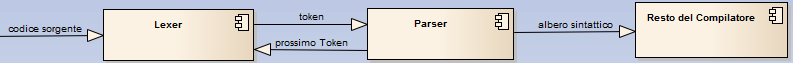
\includegraphics[height=40pt,width=420pt,scale=0.1]{files/parser.png}}
	\caption{\textit{Posizione del parser all'interno del compilatore.}}
\end{figure}
\noindent I metodi di parsing più comunemente utilizzati sono:
\begin{itemize}
	\item \textbf{Parsing top down:} la costruzione dell'albero sintattico avviene partendo dalla radice dell'albero fino ad arrivare alle foglie dell'albero;
	\item \textbf{Parsing bottom up:} la costruzione dell'albero sintattico avviene partendo dalle foglie dell'albero fino ad arrivare alla sua radice.
\end{itemize}
In questa tesi tratteremo il parsing top down in quanto il GLL parsing usa questa metodologia.
\section{Grammatiche context-free}
In questo paragrafo introduciamo le grammatiche context-free. Sono delle notazioni usate per descrivere la sintassi dei costrutti dei linguaggi di programmazione. Ad esempio in C, il while può essere definito con la seguente forma:
\begin{align}
	\textbf{while} \quad (expression) \quad statement \notag
\end{align}
Questa notazione indica che il costrutto è composto dalla parola chiave \textbf{while}, una parentesi tonda aperta, un'espressione, una parentesi tonda chiusa e uno statement. Usando la variabile \textit{expr} che indica una generica espressione e la variabile \textit{stmt} per indicare lo statement, la regola di questo costrutto può essere definita nel seguente modo:
\begin{align}\label{regolaWhile}
	stmt \to \textbf{while } ( expr ) \quad stmt 
\end{align}
La freccia può essere letta come "può avere la forma". Questa regola prende il nome di \textbf{produzione. }All'interno della produzione la parola \textit{while}, la parentesi aperta e tonda prendono il nome di \textbf{terminali}, mentre le variabili \textit{expr} e \textit{stmt} prendono il nome di \textbf{non-terminali}.
\subsection{Definizione di grammatica}
Una grammatica context-free è una quadrupla i cui elementi sono \cite{libro: compilatori}:
\begin{enumerate}
	\item \textbf{Terminali. }I terminali sono simboli di base con cui la grammatica definisce il linguaggio. Il termine "\textit{token}" è un sinonimo di terminale.
	\item \textbf{Non-Terminali. }I non-terminali sono variabili sintattiche che denotano un insieme di stringhe. Nella produzione \ref{regolaWhile} \textit{stmt} e \textit{expr} sono non-terminali. Gli insiemi di stringhe rappresentati dai non-terminali concorrono a definire il linguaggio generato dalla grammatica.
	\item \textbf{Simbolo Iniziale. }In una grammatica uno dei non-terminali costituisce il simbolo iniziale e l'insieme di stringhe che esso denota coincide con l'intero linguaggio generato dalla grammatica. 
	\item \textbf{Produzione. }Le produzioni di una grammatica definiscono come i terminali e i non-terminali possono essere combinate a formare stringhe. Ogni produzione è formata da:
	\begin{enumerate}[(a)]
		\item un non-terminale chiamato \textbf{testa}; la produzione definisce alcune delle stringhe denotate alla sua testa;
		\item il simbolo $\to$; a volte il simbolo $\Coloneqq$ è utilizzato al posto della freccia;
		\item un \textbf{ corpo } o \textbf{lato destro} costituito da zero o più non-terminali o terminali; i componenti descrivono un modo in cui le stringhe denotate dal non-terminale della testa possono essere costruite.
	\end{enumerate}
\end{enumerate}
\subsection{Convenzioni notazionali}
In questo paragrafo vengono definite le convenzioni notazionali delle grammatiche che verranno usate nel resto della tesi.
\begin{enumerate}
	\item I seguenti simboli rappresentano i terminali:
	\begin{enumerate}[(a)]
		\item le singole lettere minuscole dell'alfabeto;
		\item i simboli degli operatori matematici e di punteggiatura;
		\item le stringhe minuscole in grassetto;
		\item le cifre numeriche.
	\end{enumerate}
	\item I seguenti simboli sono non-terminali:
	\begin{enumerate}[(a)]
		\item le singole lettere maiuscole dell'alfabeto;  
		\item se usate per descrivere i singoli costrutti della programmazione, le lettere maiuscole possono indicare i non-terminali del linguaggio.
	\end{enumerate}
	\item La testa della prima produzione è il simbolo iniziale.
	\item Un insieme di produzioni del tipo \textit{A$\to$$\alpha_{1}$}, \textit{A$\to$$\alpha_{2}$}, \dots, \textit{A$\to$$\alpha_{k}$}, con una testa comune \textit{A} (che chiamiamo \textit{A-produzioni}), 
	possono essere scritte nel seguente modo: \textit{A}$\to$$\alpha_{1}$ $\mid$ $\alpha_{2}$ $\mid$ \dots $\mid$ $\alpha_{k}$. Chiamiamo $\alpha_{1}$, $\alpha_{2}$, \dots , $\alpha_{k}$ le \textit{alternative per A}.
\end{enumerate} 
\subsection{Derivazioni}
Un albero di parsing \cite{libro: compilatori} può essere costruito mediante varie fasi di derivazioni dove, partendo dal simbolo iniziale, ad ogni passo di riscrittura un simbolo non-terminale viene sostituito con il corpo di una delle sue produzione. Tale visione \textit{derivazionale} corrisponde al metodo di costruzione top-down degli alberi di parsing.
Facciamo un esempio. Consideriamo la seguente grammatica:
\begin{align}\label{grammaticaEspressioni}
	E \to EcE \mid d 
\end{align}
Un processo di derivazione, sulla stringa \textit{dcdcd} viene indicato con la seguente scrittura
\begin{align}\label{derivazione1}
	E \Rightarrow EcE \Rightarrow dcE \Rightarrow dcEcE \Rightarrow dcdcE \Rightarrow dcdcd
\end{align}
che si legge "\textit{E} deriva \textit{EcE}". La produzione \textit{E} $\to$ \textit{EcE} può essere utilizzata per sostituire qualsiasi non-terminale \textit{E} con \textit{EcE} per qualsiasi stringa di simboli della grammatica. La sequenza \ref{derivazione1} viene definita come una \textit{derivazione} della stringa \textit{dcdcd} a partire da \textit{E}. Ora diamo una definizione formale di concetto di derivazione. Sia  $\alpha$\textit{B}$\beta$ una sequenza di simboli grammaticali  dove $\alpha$ e $\beta$ sono stringhe di simboli grammaticali ed \textit{B} è un non-terminale. Supponiamo che \textit{B} $\to$ $\gamma$ sia una produzione. In tal caso possiamo scrivere $\alpha$\textit{B}$\beta$ $\Rightarrow$ $\alpha$$\gamma$$\beta$, in cui il simbolo $\Rightarrow$ significa "deriva in un solo passo". Per esprimere che una stringa "deriva in zero o più passi" una nuova stringa utilizziamo il simbolo $\overset{*}{\Rightarrow}$.\par 
\noindent Se \textit{C} $\overset{*}{\Rightarrow}$ $\alpha$, dove \textit{C} è il simbolo iniziale della grammatica \textit{G}, diciamo che $\alpha$ è una \textbf{forma sentenziale}  di \textit{G}. Una forma sentenziale può contenere sia terminali che non terminali e può essere vuota. Una \textbf{sentenza} o \textbf{frase} di \textit{G} è una forma sentenziale che non contiene nessun non-terminale. Il \textbf{linguaggio generato} da una grammatica \textit{G} è l'insieme di tutte le sue frasi. Un linguaggio che può essere generato da una grammatica è detto un \textbf{linguaggio libero dal contesto}. Se due grammatiche generano lo stesso linguaggio sono dette \textbf{equivalenti}. La stringa \textit{dcdcd} è una frase della grammatica \ref{grammaticaEspressioni} poichè esiste la derivazione \ref{derivazione1}. Le sequenze di derivazioni prevedono che ad ogni passo vengano fatte due scelte: la prima scelta consiste nello scegliere il non-terminale da sostituire; la seconda scelta consiste nello scegliere una delle produzioni in cui il non-terminale scelto risulta essere la testa della produzione. Infatti nella derivazione \ref{derivazione1} ogni non-terminale è sostituito con il corpo della produzione corrispondente. Ogni non-terminale da sostituire viene selezionato in questo modo:
\begin{enumerate}
	\item nelle \textit{derivazioni sinistre} si sceglie sempre il non-terminale più a sinistra. La derivazione \ref{derivazione1} è una derivazione a sinistra.
	\item  nelle \textit{derivazioni destre} si sceglie sempre il non-terminale più a destra. 
\end{enumerate}
\subsection{Alberi di parsing}
Un \textbf{albero di parsing} è \cite{libro: compilatori} una rappresentazione grafica di una derivazione che non dipende dall'ordine in cui le produzioni sono utilizzate per rimpiazzare i non-terminali. Ogni nodo interno rappresenta l'applicazione di una produzione ed è etichettato con il non-terminale che indica la testa della  produzione. I figli di questo nodo sono etichettati con i simboli che appaiono nel corpo della produzione utilizzata per sostituire il non-terminale. Un esempio di albero di parsing relativo alla stringa \textit{dcdcd} è mostrato nella figura \ref{fig:albero}.\par 
\begin{figure}[hbpb]
	\centering
	\begin{forest}
		[E
		[E[d]]
		[c]
		[E[E[d]][c][E[d]]]
		]
	\end{forest}
	\caption{\textit{Albero di parsing relativo alla stringa dcdcd} }\label{fig:albero}
\end{figure}
\noindent Le foglie dell'albero di parsing sono etichettate con terminali o non-terminali che, letti da sinistra verso destra formano una forma sentenziale chiamata \textbf{frontiera} dell'albero. Ora tramite un esempio mostreremo come viene costruito un albero sintattico. \par
\begin{figure}[hbpb]
	\centering
	\begin{forest}
		[E
		[E]
		[c]
		[E]
		]
	\end{forest}
	$\Rightarrow$    
	\begin{forest}
		[E
		[E[d]]
		[c]
		[E]
		]
	\end{forest}
	$\Rightarrow$    
	\begin{forest}
		[E
		[E[d]]
		[c]
		[E[E][c][E]]
		]	
	\end{forest}
	$\Rightarrow$    
	\begin{forest}
		[E
		[E[d]]
		[c]
		[E[E[d]][c][E[d]]]
		]
	\end{forest}
	\caption{\textit{Sequenza di alberi di parsing relativi alla derivazione }\ref{derivazione1}}\label{fig:passiAlbero}
\end{figure}
\noindent In figura \ref{fig:passiAlbero} viene rappresentata la sequenza di alberi sintattici costruiti dalla derivazione \ref{derivazione1}. Il primo passo della derivazione \textit{E} $\Rightarrow$ \textit{EcE} prevede di aggiungere come radice dell'albero sintattico il simbolo iniziale \textit{E} e come figli \textit{E}, \textit{c} ed \textit{E} che corrisponde al corpo di produzione \textit{EcE}. Al secondo passo della derivazione \textit{E} $\Rightarrow$ \textit{d} aggiungiamo al nodo più a sinistra \textit{E} il nodo figlio \textit{d}. Così facendo otteniamo all'utimo passo il corrispondente albero sintattico per la stringa \textit{dcdcd}.
\subsection{Ambiguità}
Una grammatica viene definita \textbf{ambigua} se produce più di un albero sintattico. In altre parole una grammatica ambigua presenta \cite{libro: compilatori} più di una derivazione destra o sinistra per una frase. Facciamo un esempio. Prendiamo in considerazione la grammatica \ref{grammaticaEspressioni} e la frase \textit{dcdcd}; questa frase presenta due alberi di parsing che sono:\par
\begin{figure}[hbpb]\label{alberibis}
	\centering
	\begin{forest}
	[E
	[E[d]]
	[c]
	[E[E[d]][c][E[d]]]
	]
	\end{forest}
	\begin{forest}
	[E
	[E[E[d]][c][E[d]]]
	[c]
	[E[d]]
	]
	\end{forest}
	\caption{\textit{Alberi di parsing generati da una grammatica ambigua}}
\end{figure}
\noindent Di conseguenza risulta che la grammatica \ref{grammaticaEspressioni} risulta essere ambigua.
\subsection{Grammatiche ricorsive}\label{par:ric}
Una grammatica viene definita \textbf{ricorsiva} \cite{libro: compilatori} se ha un non-terminale \textit{A} per cui esiste una derivazione del tipo \textit{A}$\overset{+}{\Rightarrow}$ \textit{A}$\alpha$ o \textit{A}$\overset{+}{\Rightarrow}$ $\alpha$\textit{A} della stringa $\alpha$. La prima derivazione è chiamata \textbf{ricorsione a sinistra}, la seconda è chiamata \textbf{ricorsione a destra}. Un esempio di ricorsione a sinistra è la seguente produzione:
\[
	stmt \to stmt; expr
\]
Le grammatiche ricorsive risultano essere problematiche da gestire dai parser a discesa ricorsiva perchè entrano in un ciclo infinito. Supponiamo di voler applicare questa produzione; la prima cosa che facciamo è invocare la procedura \textit{stmt()} che corrisponde al suo primo simbolo. Essendo che il corpo della produzione inizia con \textit{stmt} la procedura \textit{stmt()} viene invocata ricorsivamente. Poichè il simbolo in input cambia solo quando si verifica una corrispondenza con un terminale del corpo della produzione, succederà che il parser continuerà a leggere sempre lo stesso simbolo. Di conseguenza la procedura \textit{stmt()} viene chiamata una seconda volta così come la prima fino all'infinito.
\section{Parsing top down}
Il parsing top down è una tecnica che prevede di costruire l'albero di parsing per una determinata stringa partendo dalla radice dell'albero fino ad arrivare alle foglie che rappresentano i simmboli della stringa. Questo parsing effettua derivazioni a sinistra sulle stringhe che analizza. Infatti ad ogni passo di computazione il parsing top down cerca di trovare un possibile corpo di produzione da sostituire ad ogni non-terminale. Una volta fatto ciò cerca di trovare una corrispondenza tra i simboli della stringa in ingresso e tra i simboli del corpo della produzione. In questo paragrafo analizzeremo i principi e il funzionamento del parsing top down. Verranno presentati i seguenti argomenti: parser a discesa ricorsiva, le funzioni FIRST e FOLLOW che vengono utilizzate per scegliere le produzioni da sostituire basandosi sul simbolo in input che si sta analizzando, le grammatiche LL(1) e i parser predittivi non ricorsivi.
\subsection{Parsing a discesa ricorsiva}
Un parsing a discesa ricorsiva è un programma che contiene una procedura per ogni non-terminale della grammatica. L'esecuzione \cite{libro: compilatori} inizia con la procedura relativa al simbolo iniziale e termina con successo se il suo corpo scandisce tutta la stringa d'ingresso. Una procedura per un non-terminale viene mostrato nella figura 2.5.
\begin{figure}[hbpb]
	%\flushleft
	1) \textbf{void} \textit{A}()$\{$\par
	2)\hspace{0.5cm}Scegli, per \textit{A}, una produzione \textit{A} $\to$ $X_1$, $X_2$ \dots $X_k$;\par
	3)\hspace{0.5cm}\textbf{for}(\textit{i} da 1 fino a \textit{k})$\{$\par
	4)\hspace{1.1cm}\textbf{if}($X_i$ è non-terminale)$\{$\par
	5)\hspace{1.4cm}richiama la procedura $X_i$();\par
	6)\hspace{1.1cm}$\}$\par		
	7)\hspace{1.1cm}\textbf{else}$\{$\par	
	8)\hspace{1.3cm}\textbf{if}($X_i$ è uguale al simbolo d'ingresso corrente a)$\{$\par
	9)\hspace{2.0cm}procedi al simbolo successivo nella sequenza d'ingresso;\par
   10)\hspace{1.3cm}$\}$\par
   11)\hspace{1.4cm}\textbf{else}$\{$/* si è verificato un errore */;$\}$\par
   12)\hspace{0.5cm}$\}$\par
   13) $\}$\par
	\caption{\textit{Procedura di un non-terminale per un parser top down \cite{libro: compilatori}}}\label{fig:code}
\end{figure}

\noindent Lo pseudocodice mostrato \cite{libro: compilatori} in questa figura è non deterministico poichè inizia con la scelta di quale produzione utilizzare per \textit{A} senza indicare come deve essere fatta la scelta. Questo metodo può richiedere backtracking, cioè può richiedere di rileggere più di una volta la stringa in ingresso. In pratica, questa tecnica, viene utilizzata raramente per i costrutti dei linguaggi di programmazione e quindi risulta difficile trovare parser che la usano. Una grammatica ricorsiva risulta essere compromettente per questo tipo di parser in quanto può entrare in un ciclo infinito. Per maggiori dettagli si veda il paragrafo \ref{par:ric}
\subsection{Funzioni FIRST e FOLLOW}
Per stabilire quale produzione applicare per sostituire un non-terminale basandoci sui simboli della stringa in input, i parser, sia quelli top-down e bottom-up, usano le funzioni FIRST e FOLLOW.\par
Definiamo \textbf{FIRST}($\alpha$), \cite{libro: compilatori} in cui $\alpha$ è una generica stringa di simboli della grammatica, come l'insieme dei terminali che costituiscono l'inizio delle stringhe derivabili da $\alpha$. Se $\alpha$ $\overset{*}{\Rightarrow}$ $\epsilon$, allora anche $\epsilon$ appartiene all'insieme FIRST.\par
Definiamo \textbf{FOLLOW}(\textit{A}), in cui \textit{A} è un non-terminale, come l'insieme dei simboli terminali che possono apparire immediatamente alla destra di \textit{A}in qualche forma sentenziale, cioè l'insieme dei terminali \textit{a} per cui esiste una derivazione nella forma \textit{A} $\overset{*}{\Rightarrow}$ $\alpha$\textit{Aa}$\beta$, dove $\alpha$ e $\beta$ sono generiche forme sentenziali. Se \textit{A} appare come simbolo più a destra di una forma sentenziale, allora $\$$ appartiene al FOLLOW(\textit{A}).\par 
\noindent Facciamo un esempio di come si calcolano FIRST e FOLLOW su una grammatica. Consideriamo la seguente grammatica:
\begin{align}\label{grammatica2}
	I  & \to A \notag \\
	A  & \to S \notag \\ 
	S  & \to CC \notag \\
	C  & \to cC \mid d 
\end{align}
I FIRST e FOLLOW di questa grammatica sono:
\begin{enumerate}
	\item FIRST(\textit{I})=FIRST(\textit{A})=FIRST(\textit{S})=FIRST(\textit{C})=$\{$c,d$\}$. Per capire il motivo di ciò, si noti che le due produzioni per \textit{C} hanno i corpi che iniziano con i due simboli terminali c e d. Poichè \textit{S}, ha solo una produzione che inizia per \textit{C} e non deriva $\epsilon$, il FIRST(\textit{S}) coincide con FIRST(\textit{C}). Lo stesso ragionamento lo si può applicare per FIRST(\textit{S}) e FIRST(\textit{A})
	\item FOLLOW(\textit{I})=FOLLOW(\textit{A})=FOLLOW(\textit{S})=$\{$$\$$$\}$. Dato che \textit{I} è il simbolo iniziale, il FOLLOW(\textit{I}) deve contenere il carattere speciale $\$$. Poichè \textit{S} e \textit{A} appaiono da sole nel corpo di altre produzioni nè consegue che sono seguite dal simbolo di fine stringa $\$$. Pertanto il  FOLLOW(\textit{A}) e  FOLLOW(\textit{S}) coincide con il  FOLLOW(\textit{I}).
	\item FOLLOW(\textit{C})=$\{$c,d,$\$$$\}$. All'interno di una produzione il simbolo \textit{C} è seguito da un altro simbolo \textit{C}. Pertanto il FOLLOW(\textit{C}) include i simboli del FIRST(\textit{C}). Inoltre essendo che il simbolo \textit{C} risulta essere l'ultimo simbolo all'interno di una produzione allora il simbolo $\$$ rientra nel FOLLOW(\textit{C}).
\end{enumerate}
\subsection{Grammatiche LL(1)}
Un parser predittivo viene sempre costruito a partire da una grammatica della classe LL(1). La prima L \cite{libro: compilatori} indica che la stringa in input che si sta analizzando viene letta da sinistra verso destra. La seconda L specifica che viene fatta una derivazione a sinistra; infine l'1 fra le parentesi indica che le decisioni del parser vengono fatte analizzando un solo simbolo di lookhead. Data una grammatica G con due produzioni \textit{A} $\to$ $\alpha$ $\mid$ $\beta$ è definita LL(1) se sono verificate le seguenti condizioni:
\begin{itemize}
	\item FIRST($\alpha$) e FIRST($\beta$) risultano essere insiemi disgiunti.
	\item Se $\epsilon$ appartiene a FIRST($\beta$) allora FIRST($\alpha$) e FOLLOW(\textit{A}) sono insiemi disgiunti; la stessa cosa vale se $\epsilon$ appartiene a FIRST($\alpha$).
\end{itemize}
In base a ciò, un parser predittivo per una grammatica LL(1) può essere sempre costruito se è possibile sostituire un non-terminale con una sola produzione che viene scelta in base al simbolo di input corrente. Ovviamente nessuna grammatica ambigua e ricorsiva può essere una grammatica LL(1). L'algoritmo seguente raccoglie le informazioni di FIRST e FOLLOW in una \textbf{tabella di parsing predittivo} \textit{M}[\textit{A},\textit{a}], dove \textit{A} è un non-terminale e \textit{a} è un terminale. A volte può essere anche il marcatore di fine sequenza $\$$. L'algoritmo sceglie la produzione \textit{A}$\to$ $\alpha$ per un simbolo \textit{a} solo se il simbolo appartiene a FIRST($\alpha$). Quando invece abbiamo a che fare con derivazioni \textit{a} $\overset{*}{\Rightarrow}$ $\epsilon$, scegliamo sempre la produzione \textit{A} $\to$ $\alpha$ se il simbolo corrente appartiene al FOLLOW(\textit{A}), oppure se si è raggiunto il simbolo $\$$ nella stringa in input e se tale simbolo appartiene a FOLLOW(\textit{A}). Se dopo questi passi non vi è alcuna produzione per \textit{M}[\textit{A},\textit{a}], si ha una condizione di errore, che viene indicata vuota nella casella corrispondente. Una grammatica ricorsiva o ambigua presenta più produzioni per un simbolo in input.\par 
\noindent Facciamo un esempio e prendiamo in riferimento la grammatica \ref{grammatica2}. Applichiamo l'algoritmo precedente ed otteniamo la tabella di parsing.\par
\begin{table}
	\centering
	\label{tabellaparsing}
	\begin{tabular}{ccccc} %\hline 
		\toprule
		%\multirow{2}*{\textbf{Non Terminale}} & %\multicolumn{4}{c}{\textbf{Simbolo d'ingresso}} \\ 
		%\cmidrule(lr){2-4}
		& \textbf{c} & \textbf{d} & \textbf{$\$$} \\ 
		\midrule
		\textbf{I}			& \textit{I} $\to$ \textit{A}  & \textit{I} $\to$ \textit{A} &    \\ 
		\textbf{A} 			& \textit{A} $\to$ \textit{S}  & \textit{A} $\to$ \textit{S} &    \\ 
		\textbf{S}			& \textit{S} $\to$ \textit{CC} & \textit{S} $\to$ \textit{CC} &   \\ 
		\textbf{C} 			& \textit{C} $\to$ \textit{cC}& \textit{C} $\to$ \textit{d} &     \\ 
		\bottomrule
	\end{tabular}
	\caption{\textit{Tabella di parsing della grammatica }\ref{grammatica2}}
\end{table} 
\vspace{1.5cm}
\noindent Si consideri, per esempio la produzione \textit{I} $\to$ \textit{A}. Dato che FIRST(\textit{A}) = FIRST(\textit{S}) questa produzione viene aggiunta sia {\textit{M}[\textit{A},\textit{c}] e a {\textit{M}[\textit{A},\textit{d}]. Le caselle vuote in corrispondenza del simbolo $\$$ indicano gli errori.
\subsection{Parsing predittivo non ricorsivo}
Un parser predittivo non ricorsivo \cite{libro: compilatori} viene costruito usando uno stack, piuttosto che effettuare le chiamate ricorsive. Se \textit{w} è la porzione dell'ingresso riconosciuta a un certo momento, allora lo stack contiene una sequenza di simboli grammaticali $\alpha$ tali che \textit{S} $\overset{*}{\Rightarrow}$ \textit{w}$\alpha$. Questo parser usa un buffer d'ingresso, che contiene la stringa da analizzare compreso anche il simbolo $\$$ per segnare la fine della stringa, uno stack che contiene i simboli grammaticali e la tabella di parsing descritta al paragrafo precedente. Il fondo dello stack viene segnalato con il simbolo $\$$. Il parser funziona nel seguente modo:
\begin{enumerate}
	\item riceve in input una stringa \textit{w} e una tabella di parsing \textit{M} relativa ad una grammatica \textit{G};
	\item \label{PASSO} ad ogni passo di computazione si controlla un simbolo \textit{X} in cima allo stack e un simbolo \textit{a} della stringa \textit{w} in input.
	\item Se \textit{X} è un non-terminale, il parser lo sostituisce con il corpo della produzione che si trova nella posizione \textit{M}[\textit{X},\textit{a}].
	\item Altrimenti, se \textit{X} è un terminale, allora il parser verifica la corrispondenza di \textit{X} con un simbolo della stringa \textit{w} e se esiste legge il simbolo successivo.
	\item Ripetere le operazioni dal passo \ref{PASSO}.
	\item Il parser termina con successo se lo stack non contiene nessun simbolo \textit{X} e ciò determina che la stringa letta fa parte della grammatica \textit{G}.
\end{enumerate}

\vspace{0.5cm}
\begin{table}
	\centering
	\label{tabellaStack}
	\begin{tabular}{cclc}
		\toprule
		\textbf{Input} & \textbf{Stack} & \textbf{Azione} & \textbf{Riconosciuta}\\
		\midrule
		\textbf{cdd$\$$} & \textit{I$\$$}  \\
		\textbf{cdd$\$$} & \textit{A$\$$}  & output \textit{I} $\to$ \textit{A} \\
		\textbf{cdd$\$$} & \textit{S$\$$}  & output \textit{A} $\to$ \textit{S} \\
		\textbf{cdd$\$$} & \textit{CC$\$$}  & output \textit{S} $\to$ \textit{CC} \\
		\textbf{cdd$\$$} & \textit{cCC$\$$}  & output \textit{C} $\to$ \textit{cC} \\
		\textbf{dd$\$$} & \textit{CC$\$$}  & consuma \textbf{c} & \textbf{c}\\
		\textbf{dd$\$$} & \textit{dC$\$$}  & output \textit{C} $\to$ \textit{d} & \textbf{c}\\
		\textbf{d$\$$} & \textit{C$\$$}  & consuma \textbf{d} & \textbf{cd}\\
		\textbf{d$\$$} & \textit{d$\$$}  & output \textit{C} $\to$ \textit{d} & \textbf{cd}\\
		\textbf{$\$$} & \textit{$\$$}  & consuma \textbf{d} & \textbf{cdd}\\
		\bottomrule
	\end{tabular}
	\caption{\textit{Mosse di un parser predittivo sulla stringa \textbf{cdd}} }
\end{table}
\noindent Nella tabella 2.2 vengono riportate le mosse del parser predittivo applicate alla grammatica \ref{grammatica2}. La cima dello stack è riportata a sinistra nella colonna "Stack". Tali mosse corrispondono alla derivazione sinistra; infatti abbiamo che:
\begin{align}
I \Rightarrow A \Rightarrow S \Rightarrow CC \Rightarrow cCC \Rightarrow cdC \Rightarrow cdd \notag
\end{align}
Si noti che le forme sentenziali in tale derivazione corrispondono alla porzione di stringa in input già analizzata (indicata nella colonna "Riconosciuta").
\section{Conclusioni}
In questo capitolo è stato discusso di come funziona il parsing top down ed in particolare si è discusso degli algoritmi di parsing LL(1). Questo parser, però, presenta dei limiti:
\begin{itemize}
	\item Non sono adatti per grammatiche ambigue e ricorsive;
	\item Non ammettono tabelle di parsing in cui vi sono più produzioni per un simbolo d'ingresso.
\end{itemize}
Delle possibili soluzioni a questi limiti prevedono: l'eliminazione dell'ambiguità e della ricorsione dalla grammatica, l'uso della fattorizzazione a sinistra per rendere la grammatica più adatta al parsing predittivo o l'uso di parsing generalizzati top down che usano il non-determinismo per superare i conflitti che trova un parser predittivo nelle tabelle di parsing. Nel capitolo successivo discuteremo di quest'ultima soluzione.
	\chapter{GLL Parsing}\label{cap2}
\section{Introduzione}
Nel capitolo precedente abbiamo discusso i concetti e il funzionamento del parsing su grammatiche LL(1). In questo capitolo discuteremo di un estensione di questo parsing, chiamato \textbf{Parsing LL Generalizzato (GLL)}. Questo parsing è un parser a discesa ricorsiva ed è adatto a gestire tutte le grammatiche comprese quelle che risultano essere ambigue e ricorsive. In questo capitolo vedremo come questo parser supera i limiti che hanno i parser LL(1) e ne mostreremo i concetti base di questo parsing e il suo funzionamento.
\section{Stack e descrittori elementari}\label{par1}
In questo paragrafo discuteremo del funzionamento base del GLL Parsing \footnote{Gli algoritmi e gli esempi presenti in questo paragrafo sono riconducibili alla bibliografia \cite{pubblicazione: scott}}. Data la seguente grammatica:
\begin{align}\label{gram3}
	S & \to ASd \mid BS \mid \epsilon \notag \\
	A & \to a \mid c \notag \\
	B & \to a \mid b 
\end{align}
Un parser a discesa ricorsiva \cite{pubblicazione: scott} è composto dalle seguenti funzioni: $p_S$(), $p_A$(), $p_B$(), la funzione principale \textit{main}() e la funzione per segnalare gli errori \textit{error}(). Ogni funzione contiene codice per ogni alternativa, $\alpha$, e verificano che il simbolo corrente della stringa in input appartiene a FIRST($\alpha$) o al FOLLOW($\alpha$). La stringa in input viene rappresentata come un array globale \textit{I} di lunghezza \textit{m}+1, dove \textit{I}[\textit{m}]=$\$$, segnala la fine della stringa. L'implementazione del parser viene rappresentata di seguito.\\
main()$\{$ \textit{i} = 0 \par
\hspace{1cm}\textbf{if}(\textit{I}[\textit{i}] $\in$ $\{$\textit{a, b, c, d,$\$$}$\}$)$\{$ $p_S$(); \textbf{else} \textit{error}();\par
\hspace{1cm}\textbf{if}(\textit{I}[\textit{i}] = $\$$)$\{$ report success $\}$ \textbf{else} \textit{error}()\\	
$\}$\\
$p_S$()$\{$ \par
\hspace{0.5cm}\textbf{if}(\textit{I}[\textit{i}] $\in$ $\{$\textit{a, c}$\}$)$\{$ $p_A$(); $p_S$(); \textbf{if}(\textit{I}[\textit{i}] = \textit{d})$\{$ \textit{i} = \textit{i} + 1; $\}$ \textbf{else} \textit{error}(); $\}$\par
\hspace{0.5cm}\textbf{if}(\textit{I}[\textit{i}] $\in$ $\{$\textit{a, b}$\}$)$\{$ $p_B$(); $p_S$(); $\}$ $\}$\\
$p_A$()$\{$ \par
\hspace{0.5cm}\textbf{if}(\textit{I}[\textit{i}] = \textit{a})$\{$ \textit{i} = \textit{i} + 1;$\}$\par \hspace{0.5cm}\textbf{else} \textbf{if}(\textit{I}[\textit{i}] = \textit{c})$\{$ \textit{i} = \textit{i} + 1 $\}$ \textbf{else} \textit{error}(); $\}$\\
$p_B$()$\{$ \par \hspace{0.5cm}\textbf{if}(\textit{I}[\textit{i}] = \textit{a})$\{$ \textit{i} = \textit{i} + 1; $\}$\par \hspace{0.5cm}\textbf{else} \textbf{if}(\textit{I}[\textit{i}] = \textit{b})$\{$ \textit{i} = \textit{i} + 1 $\}$ \textbf{else} \textit{error}(); $\}$\par
\vspace{0.3cm}
Questa è la tabella di parsing della grammatica \ref{gram3}.
\begin{table}[hbpb]
	\centering
	\label{tabellaparsingNLL1}
	\begin{tabular}{cccccc} 
		\toprule
		%\multirow{2}*{\textbf{Non Terminale}} & %\multicolumn{4}{c}{\textbf{Simbolo d'ingresso}} \\ 
		%\cmidrule(lr){2-4}
		& \textbf{a} & \textbf{b} & \textbf{c} & \textbf{d} &\textbf{$\$$} \\ 
		\midrule
		\textbf{S} 	& \textit{S}$\to$\textit{ASd} $\mid$ \textit{BS} & \textit{S}$\to$\textit{BS}&\textit{S}$\to$ \textit{ASd}&\textit{S}$\to$$\epsilon$& \textit{S}$\to$$\epsilon$\\ 
		\textbf{A} & \textit{A}$\to$\textit{a}&  & \textit{A}$\to$\textit{c}\\ 
		\textbf{B} & \textit{B}$\to$\textit{a} & \textit{B}$\to$\textit{b}&   \\ 
		\bottomrule
	\end{tabular}
	\caption{\textit{Tabella di parsing della grammatica }\ref{gram3}}
\end{table} \par
Da quello che si può notare dalla tabella \ref{gram3} questa grammatica non è LL(1) in quanto è presente un conflitto e di conseguenza l'algoritmo implementato non funziona correttamente. Affinchè l'algoritmo funzioni correttamente è necessario utilizzare il non determinismo. Per fare ciò dobbiamo convertire le chiamate a funzioni con operazioni di \textbf{push} su uno stack e utilizzare i \textbf{goto} per spostarci sulle varie partizioni delle funzioni. Partizioniamo in varie parti i corpi delle funzioni il cui non-terminale non è LL(1) ed attribuiamo un etichetta ad ogni partizione. Per registrare le possibili scelte che il parser può fare per sostituire un non-terminale utilizziamo dei \textbf{descrittori} e sostituiamo il punto in cui termina l'algoritmo con l'esecuzione di un descrittore successivo. Le funzioni d'errore vengono sostituite con l'esecuzione di descrittori successivi. Il nuovo punto di termine sarà quando non esistono più descrittori da eseguire. Formalmente un \textbf{descrittore elementare} è una tripla (\textbf{L,s,j}) dove \textbf{L} è un etichetta di una partizione, \textbf{s} è uno stack e \textbf{j} è la posizione nell'array \textit{I}. Questi descrittori li manteniamo in un insieme \textbf{R}. Ogni volta che si verifica la fine di una funzione di parsing e ad ogni punto in cui è presente un non-terminale non LL(1) (quindi siamo in presenza di non-determinismo) all'interno dell'algoritmo, creiamo un nuovo descrittore che è formato dall'etichetta in cima allo stack corrente. Quando l'algoritmo di parsing trova un simbolo dell'input \textit{I}[\textit{i}] diciamo che l'etichetta \textit{L} in cima allo stack è estratto dallo stack \textit{s}=[\textit{s$^{'}$},\textit{L}] e (\textit{L,s$^{'}$,i}) viene aggiunta a \textbf{R}. Questa azione viene denotata con la funzione \textit{pop(s,i,\textbf{R})}. Dopo aver fatto ciò rimuoviamo il descrittore (\textit{L$^{'}$,t,j}) da \textbf{R} e l'algoritmo riparte dall'etichetta \textit{L$^{'}$}, con stack \textit{t} e con il simbolo in input \textit{I}[\textit{j}]. L'algoritmo termina quando l'insieme \textbf{R} è vuoto. Useremo la notazione \textit{L}$^{k}$ per unire l'etichetta \textit{L} e l'indice \textit{k} che indica il simbolo corrente nell'input \textit{I}; mentre lo stack vuoto viene denotato con [ ]. Lo stack \textit{s} viene aggiornato con la funzione \textit{push(s, L$^{k}$)}; questa funzione non fa altro che aggiungere  l'elemento \textit{L}$^{k}$ in cima allo stack. Di seguito viene presentato l'algoritmo.\par
\vspace{0.5cm}
\hspace{0.2cm}\textit{i} = 0; \textbf{R} = $\emptyset$; \textit{s} = [\textit{L$_0^{0}$}];\\
$L_S$: \textbf{if}(\textit{I}[\textit{i}] $\in$ $\{$\textit{a,c}$\}$) add($L_{S1}$, \textit{s, i}) to \textbf{R} \par
\hspace{0.2cm}\textbf{if}(\textit{I}[\textit{i}] $\in$ $\{$\textit{a,b}$\}$) add(\textit{$L_{S2}$}, \textit{s, i}) to \textbf{R}\par
\hspace{0.2cm}\textbf{if}(\textit{I}[\textit{i}] $\in$ $\{$\textit{d,$\$$}$\}$) add(\textit{$L_{S3}$}, \textit{s, i}) to \textbf{R} \\
$L_0$: \textbf{if}(\textbf{R} $\ne$ $\emptyset$)$\{$ remove(\textit{L}, $s_1$, \textit{j}) from \textbf{R} \par
\hspace{2.2cm}\textbf{if}(\textit{L} = $L_0$ and $s_1$ = [ ] and \textit{j} = |\textit{I}|) report success \par
\hspace{2.2cm}\textbf{else}$\{$ \textit{s} = $s_1$; \textit{i} = \textit{j}; \textbf{goto} \textit{L} $\}$ \\
$L_{S1}$: \textit{push}(\textit{s, L$_1^{i}$}); \textbf{goto} $L_A$\\
$L_1$:  \textit{push}(\textit{s, L$_2^{i}$}); \textbf{goto} $L_S$\\
$L_2$:  \textbf{if}(\textit{I}[\textit{i}] = \textit{a})$\{$ \textit{i} = \textit{i} + 1; \textit{pop}(\textit{s}, \textit{i}, \textbf{R});$\}$ \textbf{goto} $L_0$ \\
$L_{S2}$: \textit{push}(\textit{s, L$_3^{i}$}); \textbf{goto} $L_B$\\
$L_3$:  \textit{push}(\textit{s, L$_4^{i}$}); \textbf{goto} $L_S$\\
$L_4$: \textit{pop}(\textit{s, i}, \textbf{R}); \textbf{goto} $L_0$ \\
$L_{S3}$: \textit{pop}(\textit{s, i}, \textbf{R}); \textbf{goto} $L_0$ \\
$L_A$:  \textbf{if}(\textit{I}[\textit{i}] = \textit{a})$\{$ \textit{i} = \textit{i} + 1; \textit{pop}(\textit{s, i}, \textbf{R});$\}$ \textbf{goto} $L_0$ $\}$ \par
\hspace{0.2cm} \textbf{else}$\{$ \textbf{if}(\textit{I}[\textit{i}] = \textit{c})$\{$ \textit{i} = \textit{i} + 1; \textit{pop}(\textit{s, i}, \textbf{R});$\}$ \par 
\hspace{1.5cm}\textbf{goto} $L_0$ $\}$ \\
$L_B$:  \textbf{if}(\textit{I}[\textit{i}] = \textit{a})$\{$ \textit{i} = \textit{i} + 1; \textit{pop}(\textit{s, i}, \textbf{R});$\}$ \textbf{goto} $L_0$ $\}$ \par
\hspace{0.2cm} \textbf{else}$\{$ \textbf{if}(\textit{I}[\textit{i}] = \textit{b})$\{$ \textit{i} = \textit{i} + 1; \textit{pop}(\textit{s, i}, \textbf{R});$\}$ \par
\hspace{1.5cm}\textbf{goto} $L_0$ $\}$ \par 
\vspace{0.3cm}
Ora facciamo un esempio usando la stringa d'input \textit{aad}$\$$. Incomiciamo la nostra computazione aggiungendo prima la tripla (L$_{S1}$,[L$_0^{0}$],0), e poi la tripla (L$_{S2}$,[L$_0^{0}$],0) ad \textbf{R} ed andiamo all'etichetta L$_0$. Rimuoviamo (L$_{S1}$,[L$_0^{0}$],0) da \textbf{R} ed andiamo alla linea con etichetta L$_{S1}$. L'operazione di \textit{push} aggiunge allo stack \textit{s} [L$_0^{0}$,L$_1^{0}$] ed andiamo in L$_A$. In L$_A$ abbiamo che il parser ha trovato una coincidenza con il simbolo \textit{a}, incrementa l'indice \textit{i} per leggere il simbolo successivo, fa un operazione di \textit{pop} ed aggiunge  (L$_{1}$,[L$_0^{0}$],1) ad \textbf{R} e ritorna in L$_0$. Allo stesso modo processiamo  (L$_{S2}$,[L$_0^{0}$],0) da \textbf{R} e alla fine avremo (L$_{3}$,[L$_0^{0}$],1) che viene aggiunto ad \textbf{R}. Quindi \textbf{R} risulterà avere le seguenti triple:
\begin{align}
	\textbf{R} = \{ (L_1,[L_0^{0}],1), (L_3,[L_0^{0}],1) \} \notag
\end{align}
Successivamente estraiamo (L$_{1}$,[L$_0^{0}$],1) e lo processiamo. Alla linea L$_1$ facciamo un \textit{push} sullo stack \textit{s} [L$_0^{0}$,L$_2^{1}$] ed andiamo alla linea con etichetta L$_S$ e aggiungiamo (L$_{S1}$,[L$_0^{0}$,L$_2^{1}$],1) e (L$_{S2}$,[L$_0^{0}$,L$_2^{1}$],1) ad \textbf{R}. Allo stesso modo processiamo (L$_{3}$,[L$_0^{0}$],1) e in \textbf{R} abbiamo:
\begin{align}
	\textbf{R} = \{ (L_{S1},[L_0^{0},L_2^{1}],1), (L_{S2},[L_0^{0},L_2^{1}],1), (L_{S1},[L_0^{0},L_4^{1}],1), (L_{S2},[L_0^{0},L_4^{1}],1) \} \notag
\end{align}
Processando ognuno di questi elementi otteniamo:
\begin{align}
	\textbf{R} = \{ (L_{1},[L_0^{0},L_2^{1}],2), (L_{3},[L_0^{0},L_2^{1}],2), (L_{1},[L_0^{0},L_4^{1}],2),  (L_{3},[L_0^{0},L_4^{1}],2) \} \notag
\end{align}
Quando l'input risulta essere \textit{I}[\textit{i}] = \textit{d} e processiamo queste triple otteniamo che in \textbf{R} abbiamo:
\begin{align}
	\textbf{R} = \{ (L_{S3},[L_0^{0},L_2^{1},L_2^{2}],2), (L_{S3},[L_0^{0},L_2^{1},L_4^{2}],2),  (L_{S3},[L_0^{0},L_4^{1},L_2^{2}],2), (L_{S3},[L_0^{0},L_4^{1},L_4^{2}],2) \} \notag
\end{align}
Processando di nuovo questi elementi otteniamo:
\begin{align}
	\textbf{R} = \{ (L_{2},[L_0^{0},L_2^{1}],2), (L_{4},[L_0^{0},L_2^{1}],2), (L_{2},[L_0^{0},L_4^{1}],2) (L_{4},[L_0^{0},L_4^{1}],2) \} \notag
\end{align}
Da queste triple otteniamo:
\begin{align}
 	\textbf{R} = \{ (L_{2},[L_0^{0}],3), (L_{2},[L_0^{0}],2), (L_{4},[L_0^{0}],3), (L_{4},[L_0^{0}],2) \} \notag
\end{align}
Quando abbiamo \textit{I}[3] = $\$$ processiamo le triple mostrate precedentemente ed otteniamo la tripla (L$_{0}$,[ ],3) e la tripla (L$_{0}$,[ ],2) che vengono aggiunte ad \textbf{R} e di conseguenza l'algoritmo termina con un successo.
\section{Definizione GLL Parsing}
L'algoritmo descritto al paragrafo \ref{par1} potrebbe creare un numero esponenziale, della taglia dell'input, di descrittori per alcune grammatiche e non lavora correttamente su grammatiche ricorsive. In questo paragrafo vedremo come correggere l'algoritmo e introdurremo le nuove strutture dati utilizzate dall'nuovo algoritmo.\footnote{Le funzioni che verranno descritte nei paragrafi successivi fanno riferimento alla bibliografia \cite{pubblicazione: scott}}
\subsection{Graph structured stacks}
Nell'algoritmo presentato precedentemente, abbiamo visto che ogni volta si trovava un non-terminale non LL(1) applicavamo il non determinismo duplicando lo stack usato dal parser. Per rappresentare tutti questi stack in unica struttura dati utilizzeremo il \textbf{Graph structured stacks} (\textbf{GSS}). Viene definito \cite{tesi: lr} come un grafo diretto aciclico (DAG) i cui nodi hanno etichette L$^{k}$ che corrispondono agli elementi usati dallo stack, dove L indica un etichetta di una partizione di una funzione e \textit{k} la posizione su un simbolo della stringa in input. Questi nodi sono raggruppati in vari insiemi disgunti chiamati \textit{livelli}. Il GSS viene costruito un livello alla volta. Infatti ogni qualvolta il parser trova una coincidenza tra un simbolo in input e la grammatica crea un livello. Il GSS viene disegnato da sinistra verso destra ed il nodo più a sinitra rappresenta la cima di ogni stack. Per costruire il GSS all'interno dell'algoritmo di parsing, dobbiamo usare una nuova tripla, chiamato \textbf{descrittore}. Un descrittore è formato da (\textit{L},\textit{u},\textit{i}), dove \textit{L} è un etichetta, \textit{u} è un nodo del GSS e \textit{i} che indica la posizione di un simbolo della stringa in input \textit{I}[ ]. Queste triple vengono aggiunte ad \textbf{R}.
\subsection{Insiemi U e P}
Per stabilire l'esito del parsing è necessario usare l'insieme \textbf{U}. Questo insieme contiene gli stessi descrittori dell'insieme \textbf{R}. Questo insieme risulta necessario perchè non è possibile usare l'insieme \textbf{R}, visto che vengono rimossi tutti i descrittori creati. Un problema \cite{pubblicazione: scott} che può sorgere sia ha quando un nodo figlio \textit{w} è aggiunto ad \textit{u}, dopo aver eseguito le operazioni di pop sul GSS, perchè l'azione di pop necessita di essere applicata a questo nodo figlio. Per risolvere ciò usiamo l'insieme \textbf{P} che contiene coppie (\textit{u}, \textit{k}) e verranno utilizzate per eseguire le operazioni di pop. Infatti quando un nuovo nodo figlio \textit{w} è aggiunto ad \textit{u}, ogni elemento (\textit{u}, \textit{k}) presente in \textbf{P}, se (L$_u$, \textit{w}) non è presente in \textbf{U$_k$}, allora (L$_u$, \textit{u}, \textit{k}) è aggiunto ad \textbf{R}, dove L$_u$ è l'etichetta nel nodo \textit{u}. L'implementazione di questa tecnica verrà mostrata nel paragrafo \ref{par}  
\subsection{Funzioni fondamentali}\label{par}
L'algoritmo \cite{pubblicazione: scott} utilizza quattro funzioni che sono essenziali per il suo funzionamento. Queste funzioni vengono elencate qui di seguito.
\begin{itemize}
	\item \textbf{\textit{add()}}: La funzione \textit{add}(\textit{L}, \textit{u}, \textit{j}) controlla se c'è un descrittore (\textit{L}, \textit{u}) in U$_j$ e se non c'è lo aggiunge a U$_j$ e ad \textbf{R}. La funzione è definita nel seguente modo:\par 
	\textit{add}(\textit{L}, \textit{u}, \textit{j})$\{$ \textbf{if}((\textit{L}, \textit{u}) $\notin$ U$_j$)$\{$ add (\textit{L}, \textit{u}) to U$_j$; add (\textit{L}, \textit{u}, \textit{j}) to \textbf{R} $\}$ $\}$
	\item \textbf{\textit{pop()}}: La funzione \textit{pop}(\textit{u}, \textit{j}) chiama la funzione \textit{add}(\textit{L$_u$}, \textit{v}, \textit{j}) per tutti i figli \textit{v} di \textit{u} e aggiunge (\textit{u}, \textit{j}) a \textbf{P}. Viene definita nel seguente modo: \par
	\textit{pop}(\textit{u}, \textit{j})$\{$ \textbf{if}(\textit{u} $\ne$ \textit{u$_0$})$\{$ add (\textit{u}, \textit{j}); \par \hspace{4.1cm}\textbf{for} each child \textit{v} of \textit{u} $\{$ add (\textit{L$_u$}, \textit{v}, \textit{j}); $\}$ $\}$ $\}$
	\item \textbf{\textit{create()}}: La funzione \textit{create}(\textit{L}, \textit{u}, \textit{j}) crea un nodo \textit{v} nel GSS etichettato \textit{L}$^{j}$ con figlio \textit{u} se non esiste ancora e restituisce \textit{v}. Se (\textit{v}, \textit{k}) appartiene a \textbf{P} chiama la funzione \textit{add}(\textit{L}, \textit{u}, \textit{k}). La definizione di questa funzione è al seguente:\par 
	\textit{create}(\textit{L}, \textit{u}, \textit{j})$\{$ \textbf{if} there is not a GSS node labelled \textit{L$^{j}$} create one\par
	\hspace{3cm} let \textit{v} be the GSS node labelled \textit{L$^{j}$} \par
	\hspace{3cm} \textbf{if} there is not an edge from \textit{v} to \textit{v}$\{$ \par
	\hspace{3.6cm} create an edge from \textit{v} to \textit{u}  \par
	\hspace{3.6cm} \textbf{for all} ((\textit{v, k}) $\in$ \textbf{\textbf{P}}) $\{$ \textit{add}(\textit{L}, \textit{u}, \textit{k}) $\}$ $\}$ \par  
	\hspace{3cm} \textbf{return} \textit{v} $\}$
	\item \textbf{\textit{test()}}: La funzione \textit{test}(\textit{x}, \textit{A}, $\alpha$) controlla se il simbolo d'input corrente \textit{x} appartiene al FOLLOW(\textit{A}), dove \textit{A} è un non-terminale o appartiene al FIRST($\alpha$), dove $\alpha$ è un item che stiamo processando. \`E definita nel seguente modo:\par
	\textit{test}(\textit{x},\textit{A},$\alpha$)$\{$ \textbf{if}(\textit{x} $\in$ FIRST($\alpha$)) or ($\epsilon$ $\in$ FIRST($\alpha$) and \textit{x} $\in$ FOLLOW(\textit{A}))$\{$ \par 
	\hspace{2.6cm}\textbf{ return true } $\}$\par 
	 \hspace{2.1cm}\textbf{else} $\{$ \textbf{return false} $\}$ $\}$
\end{itemize}
\subsection{Gestione degli item}
Informalmente un \textbf{item} \cite{libro: compilatori} di una grammatica \textit{G} è una produzione di \textit{G} con un punto in qualche posizione del corpo. Ad esempio la produzione \textit{C} $\to$ \textit{DKL} ammette quattro item:
\begin{align}
	\textit{C} & \to \textit{.DKL} \notag \\
	\textit{C} & \to \textit{D.KL} \notag \\
	\textit{C} & \to \textit{DK.L} \notag \\
	\textit{C} & \to \textit{DKL.} \notag 
\end{align}
La produzione \textit{C} $\to$ $\epsilon$ genera l'item \textit{C}$\to$. .\\
Un item indica una porzione di una produzione che si sta analizzando ad un certo punto del processo di parsing. Sia $\alpha$ la parte di produzione dell'item. Nel GLL Parsing gli item verrano gestiti nel seguente modo: 
\begin{enumerate}
	\item Un item del tipo .\textit{a}$\alpha$, dove \textit{a} è un terminale, definiamo:\par
	\textit{code}(\textit{a}$\alpha$, j) = \textbf{if}(\textit{I}[\textit{j}] = \textit{a})$\{$ \textit{j} = \textit{j} + 1 $\}$ \textbf{else} $\{$ \textbf{goto} L$_0$ $\}$
	\item Un item del tipo .\textit{A}$\alpha$, dove \textit{A} è un non-terminale, definiamo:\par
	\textit{code}(\textit{A}$\alpha$, j,\textit{X}) = \textbf{if}(\textit{test}(\textit{I}[\textit{j}],\textit{X},\textit{A}$\alpha$))$\{$ \par 
	\hspace{4cm}\textit{c}$_u$ = \textit{create}(\textit{R}$_A\alpha$,\textit{c}$_u$,\textit{j}); \textbf{goto} \textit{L}$_A$ $\}$ \par 
	\hspace{3cm}\textbf{else} $\{$ \textbf{goto} L$_0$ $\}$
	\item Per la produzione \textit{A}$\to$$\epsilon$ con item \textit{C}$\to$. definiamo: \par
	\hspace{1cm}\textit{code}(\textit{A}$\to$$\epsilon$, j) = \textit{pop}(\textit{c}$_u$,\textit{j}); \textbf{goto} L$_0$;
\end{enumerate}
\vspace{0.5cm}Quindi, in base a ciò, per ogni produzione \textit{A} $\to$ $\beta$, dove $\beta$=\textit{x}$_1$$\dots$\textit{x}$_n$, abbiamo:
\begin{enumerate}
	\item Se \textit{x}$_1$ è un terminale:\par 
	\hspace{2.5cm}\textit{code}(\textit{A}$\to$$\beta$, j) = \hspace{2cm}\textit{j} = \textit{j} + 1\par
	\hspace{7.3cm} \textit{code}(\textit{x}$_2$$\dots$\textit{x}$_n$, \textit{j},\textit{A})\par
	\hspace{7.3cm} \textit{code}(\textit{x}$_3$$\dots$\textit{x}$_n$, \textit{j},\textit{A})\par
	\hspace{7.3cm} \dots \par
	\hspace{7.3cm} \textit{code}(\textit{x}$_n$, \textit{j},\textit{A})\par 
	\hspace{7.3cm} \textit{pop}(\textit{c}$_u$,\textit{j}); \textbf{goto} L$_0$;
	\item Se \textit{x}$_1$ è un non-terminale:\par 
	\hspace{2.2cm}\textit{code}(\textit{A}$\to$$\beta$, j) = \hspace{2cm} \textit{c}$_u$=\textit{create}(\textit{R}$_{Al}$,\textit{c}$_u$,\textit{j}); \textbf{goto} \textit{L}$_A$\par
	\hspace{7.1cm} $A_l$: \textit{code}(\textit{x}$_2$$\dots$\textit{x}$_n$, \textit{j},\textit{A})\par
	\hspace{7.8cm} \textit{code}(\textit{x}$_3$$\dots$\textit{x}$_n$, \textit{j},\textit{A})\par
	\hspace{7.8cm} \dots \par
	\hspace{7.8cm} \textit{code}(\textit{x}$_n$, \textit{j},\textit{A})\par 
	\hspace{7.8cm} \textit{pop}(\textit{c}$_u$,\textit{j}); \textbf{goto} L$_0$;
\end{enumerate}
\subsection{Gestione delle sostituzioni}
Siano \textit{A} $\to$ $\alpha_1$ $\mid$ $\dots$ $\mid$ $\alpha_{n}$ regole grammaticali. Quando dobbiamo gestire le sostituzioni dei non-terminali con gli opportuni corpi di produzione durante il parsing vengono definiti due modi:
\begin{enumerate}
	\item Se \textit{A} è un non-terminale LL(1) che non presenta conflitti abbiamo:\par
	\hspace{2.5cm}\textit{code}(\textit{A}, j) = \hspace{2cm}\textbf{if}(\textit{test}(\textit{I}[\textit{j}],\textit{X},$\alpha_1$)$\{$ \textbf{goto} \textit{L}$_{A1}$ $\}$ \par 
	\hspace{6.8cm} \dots \par
	\hspace{6.8cm} \textbf{else if}(\textit{test}(\textit{I}[\textit{j}],\textit{X},$\alpha_n$)$\{$\textbf{goto} \textit{L}$_{An}$$\}$ \par 
	\hspace{6.2cm} \textit{L}$_{A1}$: \textit{code}(\textit{A}$\to$$\alpha_1$, j) \par 
	\hspace{6.2cm} \dots \par 
	\hspace{6.2cm} \textit{L}$_{An}$: \textit{code}(\textit{A}$\to$$\alpha_{n}$ , j) \par 
	\item Se \textit{A} è un non-terminale non LL(1) che presenta conflitti abbiamo:\par
	\hspace{2.5cm}\textit{code}(\textit{A}, j) = \hspace{2cm}\textbf{if}(\textit{test}(\textit{I}[\textit{j}],\textit{X},$\alpha_1$)$\{$ \textit{add}(\textit{L}$_{A1}$,\textit{c}$_u$,\textit{j})$\}$ \par 
	\hspace{6.8cm} \dots \par
	\hspace{6.8cm} \textbf{else if}(\textit{test}(\textit{I}[\textit{j}],\textit{X},$\alpha_n$)$\{$ \textit{add}(\textit{L}$_{An}$,\textit{c}$_u$,\textit{j})$\}$ \par 
	\hspace{6.8cm}\textbf{goto} \textit{L}$_0$ \par 
	\hspace{6.2cm} \textit{L}$_{A1}$: \textit{code}(\textit{A}$\to$$\alpha_1$, j) \par 
	\hspace{6.2cm} \dots \par 
	\hspace{6.2cm} \textit{L}$_{An}$: \textit{code}(\textit{A}$\to$$\alpha_{n}$ , j) \par 
\end{enumerate}
\subsection{Shared packed parse forest}
Gli alberi sintattici prodotti dai vari flussi di computazione, creati dall'applicazione del non determinismo, possono essere combinati in unica struttura chiamata \textbf{Shared packed parse forest} (SPPF). I nodi padri \cite{tesi: lr} sono uniti in nuovo nodo ed un nodo involucro diventa il nodo padre di ogni sottoalbero. La grammatica \ref{grammaticaEspressioni}, che possiede due alberi di parsing, può essere rappresentata con un SPPF.\par 
\begin{figure}[hbpb]
	\centering
	\begin{forest}
	[E
	[E[d]][c][E[E[d]] [c] [E[d]]]
	[E[E[d]][c][E[d]]][c][E[d]]
	]
	\end{forest}
	\caption{\textit{SPPF relativo alla stringa dcdcd}}\label{sppf}
\end{figure}
\noindent Il GLL Parsing restituirà in output un sppf in quanto combinerà tutti gli alberi sintattici calcolati dai vari flussi di computazione creati dall'applicazione del non-determinismo. Per poter costruire questo albero sono state definite due funzioni:
\begin{itemize}
	\item \textbf{\textit{getNodeT()}}: la funzione \textit{getNodeT}($\alpha$,\textit{c}$_n$,a$x_1\dots x_n$) viene usata per inserire all'interno del sppf un nodo etichettato $\alpha$, che corrisponde ad un simbolo terminale e non, e a$x_1\dots x_n$a$x_1\dots x_n$, che equivale all'item a cui appartiene. Questo nodo creato viene collegato come nodo figlio al nodo \textit{c}$_n$. Viene definita nel seguente modo:\par
	\hspace{0.5cm}\textit{getNodeT}($\alpha$,\textit{c}$_n$,a$x_1\dots x_n$)$\{$ \textbf{for} each edge E($c_p$,$c_c$) in SPPF\par \hspace{5.5cm}\textbf{if}(($c_n$=$c_p$)and(a$x_1\dots x_n$=\textit{item of}$c_c$))$\{$ \par \hspace{5.5cm}create a new node c$_v$=(\textit{c}$_a$, a$x_1\dots x_n$);  \par 
	 \hspace{5.5cm}create an edge from \textit{c}$_n$ to \textit{c}$_v$ in SPPF;$\}\}$
	 \item \textbf{\textit{getNodeP()}}: la funzione \textit{getNodeP}(\textit{c}$_u$) viene usata per ottenere un nodo \textit{c}$_v$ padre del nodo \textit{c}$_u$ all'interno del sppf. Viene chiamata quando è necessario recuperare un non-terminale ogni volta che viene trovato un simbolo della stringa in input. In questo modo recuperiamo i restanti non-terminali del corpo di una produzione. Viene definita nel seguente modo:\par
	 \hspace{1.5cm}\textit{getNodeP}(\textit{c}$_u$)$\{$ \textbf{for} each edge E(\textit{c}$_p$,\textit{c}$_c$)in SPPF $\{$  \par 
	 \hspace{4.4cm}\textbf{if}(\textit{c}$_u$=\textit{c}$_c$)$\{$ \textbf{return} \textit{c}$_c$ $\}$ $\}$ $\}$
\end{itemize}
\section{Costruzione del GLL Parser}\label{algoritmoIntero}
Ora, avendo definito le varie funzioni e le varie operazioni da eseguire, siamo in grado di costruire in GLL Parser. Qui di seguito riportiamo lo pseudocodice del parser \footnote{Questo pseudocodice fa riferimento alla bibliografia \cite{pubblicazione: scott}. \'E stata omessa la costruzione del sppf in quanto verrà discusso nei capitoli successivi.} e nei capitoli successivi ne vedremo l'implementazione.\par 
\vspace{0.2cm}
\noindent Sia $\Gamma$ una grammatica e i suoi non-terminali sono \textit{A}, $\dots$, \textit{X}. L'algoritmo di GLL parsing per la grammatica $\Gamma$ risulta essere il seguente:\par
\vspace{0.5cm}
\noindent \textit{m} è una costante che indica la lunghezza della stringa in input\\
\textit{I} è un array che contiene la stringa in input di dimensione \textit{m}+1\\
\textit{i} è una variabile intera usata per accedere alle locazioni dell'array \textit{I}\\
GSS è un DAG che contiene i nodi etichettati nella forma \textit{L$^{j}$}\\
\textit{c}$_u$ è un nodo del GSS\\
\textbf{P} è un insieme che ha coppie formate da un nodo del GSS e di intero\\
\textbf{R} è un insieme di descrittori \par
\vspace{0.5cm}

\noindent read the input into \textit{I} and set \textit{I}[\textit{m}]=$\$$, \textit{i}=0;\\
create GSS nodes \textit{u}$_1$=\textit{L}$_0^{0}$, \textit{u}$_0$=$\$$ and edge (\textit{u}$_0$,\textit{u}$_1$)\\
\textit{c}$_u$=\textit{u}$_1$, \textit{i}=0\\
\textbf{for} 0 $\le$ \textit{j} $\le$ \textit{m} $\{$ \textbf{U$_j$} = $\emptyset$ $\}$\\
\textbf{R}=$\emptyset$, \textbf{P}=$\emptyset$\\
\textbf{goto} \textit{L}$_S$;\\
\textit{L}$_0$: \textbf{if}(\textbf{R} $\ne$ $\emptyset$)$\{$\par
\hspace{2cm} remove a descriptor (\textit{L},\textit{u},\textit{j}) from \textbf{R}\par
\hspace{2cm} \textit{c}$_u$=\textit{u}, \textit{i}=\textit{j} , \textbf{goto} \textit{L} $\}$\par
\hspace{0.1cm} \textbf{else if}((\textit{L}$_0$,\textit{u}$_0$,\textit{j}) $\in$ \textit{U}$_m$)$\{$ report success $\}$ \textbf{else}$\{$ report failure $\}$\\
\textit{L}$_A$: \textit{code}(\textit{A},\textit{i})\\
\dots \\
\textit{L}$_X$: \textit{code}(\textit{X},\textit{i})
	\backmatter
	\addcontentsline{toc}{chapter}{\\Bibliografia}
	\begin{thebibliography}{9}
\bibitem{libro: compilatori}
Alfred V.Aho, Monica S. Lam, Ravi Sethi,Jeffrey D. Ullman,
\emph{Compilatori. Principi, Tecniche e Strumenti. Seconda Edizione}. Pearson, Addison Wesley (2009). 
\bibitem{pubblicazione: scott}
Elizabeth Scott, Adrian Johnstone,
\emph{GLL Parsing}. Electronic Notes in Theorical Computer Science 253 (2010) (pp.177-189).
\bibitem{pubblicazione: tomita}
Gennaro Costagliola, Masaru Tomita, Shi-Kuo Chang,
\emph{A Generalized Parser for 2-D Languages}, IEEE (1991).
\end{thebibliography}
\end{document}